

\chapter[*高级 Transformer 与智能体架构]{*高级 Transformer 与智能体架构}\label{chap:arch}

\begin{learningbox}
本章你将了解高级的 Transformer 与智能体架构。具体而言，你将能够：
\begin{itemize}[leftmargin=*, nosep]
    \item 理解{\em 图灵完备性}的概念，并了解 Transformer 在原则上具有图灵完备性。
    \item 理解当我们用{\em 决策轨迹}（而非自然语言）训练 Transformer 模型时，它们能够进行规划。
    \item 描述在{\em 循环语言模型}中，嵌入如何能直接连到其他嵌入，从而跳过分词层。
    \item 描述智能体如何通过保存状态—动作—奖励三元组的历史，在{\em 上下文中进行强化学习}。
    \item 说明{\em 自我修改}型智能体的优势与劣势。
    \item 理解元学习如何应用于执行框架设计，以造出一个改进基础框架的{\em 元框架}。
\end{itemize}
\end{learningbox}

\section{Transformer 架构}
大语言模型的成功，催生了对 Transformer 架构若干有趣的新研究路径。大语言模型擅长语言，却不擅长推理与规划等其他类型的问题。这促使研究者去探索 Transformer 所能完成的计算类型的极限，我们将在以下几节讨论其中一些课题。具体来说，他们提出了 Transformer 是否图灵完备的问题（第~\ref{sec:turing} 节）。在规划问题上表现偏弱，促使一些研究直接用决策轨迹训练 Transformer，看这是否能让它们具备规划与回溯的能力（第~\ref{sec:decisions} 节）。接下来，我们将考察循环语言模型——多个模型在嵌入层面直接相连。


\subsection{Transformer 是图灵完备的}\label{sec:turing}
大语言模型在推理时难以管理状态，这暗示它们所能执行的计算类型是有限的。%What types of computations are transformers able to perform? %Associative next-word prediction: yes, state: no.
在理论计算机科学中，图灵完备性这一概念表明某个计算模型是否足够强大，能够执行某一类别的任何计算（其中包括正确地管理状态值）。这一概念由 Alan Turing 在 1936 年的一篇著名论文中提出，他在其中证明了某一类机器足以做到这一点 \citep{turing1936computable}。
要被称为图灵完备，一个系统必须能够模拟任何其他计算装置，并能处理任何可以用算法表达的问题（尽管可能需要无限的时间与内存）。
%In theory, a certain type of machine, the Turing machine, is capable of general computations. The Turing machine is a simple machine, consisting of a tape, a read/write head, and a memory. 
事实证明，达到图灵完备并不太难；大多数通用编程语言都是图灵完备的。\footnote{例如 Python 编程语言是图灵完备的，而不带反向引用的简单正则表达式匹配则不是。}

大语言模型——以及一般而言基于 Transformer 的模型——在管理状态上的困难，似乎暗示 Transformer 架构可能不是图灵完备的。
有趣的是，早在 2021 年 \citet{perez2021attention} 就研究了这一问题，并证明了 Transformer 架构能够模拟图灵机，因而是图灵完备的。

这是一个令人鼓舞的结果，因为它表明并不存在什么根本原因使 Transformer 无法正确地管理状态。这很可能只是找到正确提示、或找到正确预训练与微调数据集的问题。

遗憾的是，某件事在理论上可行，并不意味着实现它会很容易，也不意味着它能被高效地做到。%It may be that they must be heavily finetuned to efficiently perform certain computations. 
例如，对 Transformer 架构的某些扩展，可能会让高效的状态管理更容易实现。
下面我们讨论那些为让大语言模型能高效求解决策与规划问题而发展出来的方法。


\subsection{在决策轨迹上预训练回溯能力}\label{sec:decisions}
%\todo{delete? Goes too far? Mwa, misschien toch houden, want het idee dat je alles kunt bereiken als je er maar op traint is een krachtig idee. En wat we natuurlijk graag willen is dat ook general-language-trained LLM het kunnen. Dat is een uitdaging, dus daar gaan de andere subsecties dus over. Deze gedachte moet ik in de tekst stoppen.
Transformer 图灵完备这一发现，鼓舞了规划与决策方面的研究。
%It suggests that we only need to find a way to train or query the model in the right way in order to be able to make a decision. 
本节我们将讨论那些在决策轨迹上预训练 Transformer 架构并取得良好结果的研究。请注意，本节{\em 不是}关于在自然语言上训练的 Transformer——即大语言模型——而是关于在决策轨迹上训练的 Transformer。%In  section~\ref{sec:inferencetime} we will discuss studies that use transformers trained on natural language with inference-time methods.

\begin{figure}
    \centering
    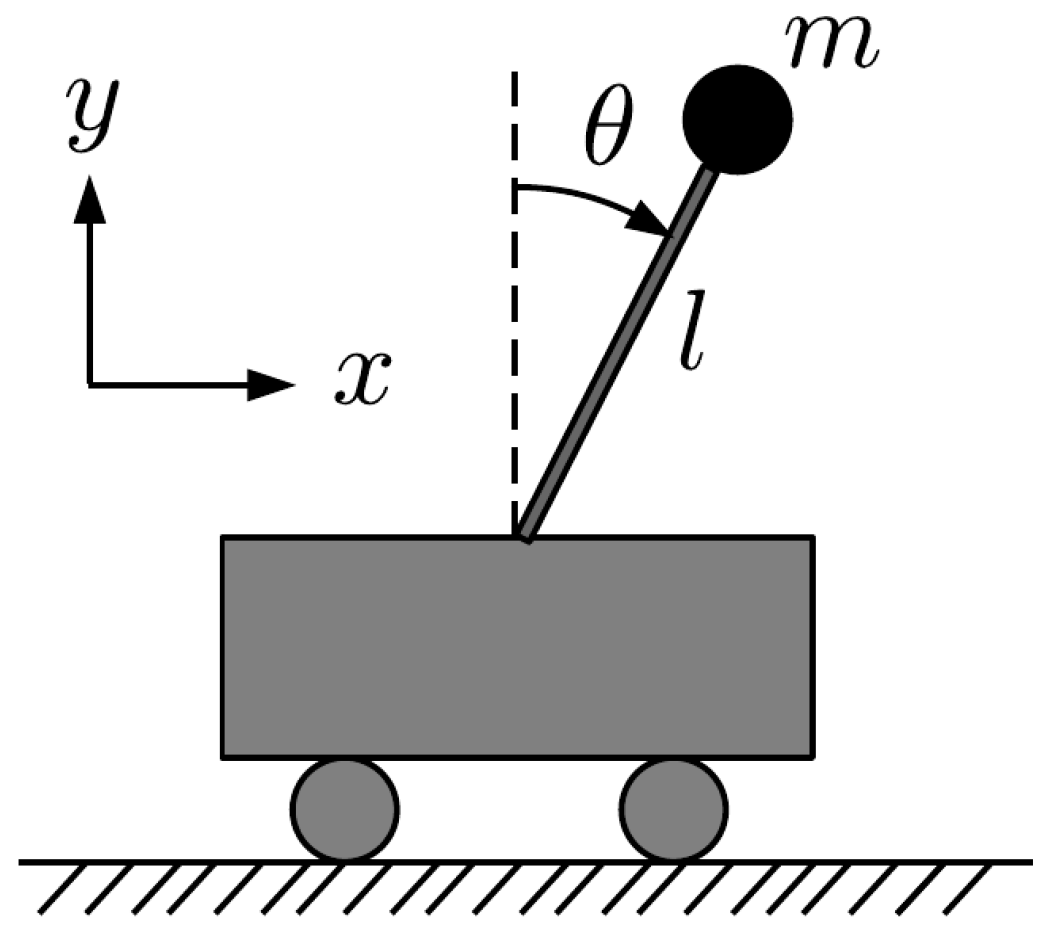
\includegraphics[width=0.5\linewidth]{figures/cartpole}
    \caption{倒立摆问题：只通过左右移动小车来保持杆子平衡}
    \label{fig:cartpole}
\end{figure}

%To see if transformers can perform planning and decision problems, 
我们首先讨论直接在决策轨迹上预训练 Transformer：决策轨迹是状态—动作—奖励三元组的序列，{\em 不是}语言 token。%, instead of first on natural language. 
%The reinforcement learning approaches that we discussed so far---React, Self Refine, Tree of Thoughts,  Reflexion---use external algorithms to manage state for the prompt improvement loop. A perhaps more elegant solution would be to perform reinforcement learning fully in-context, within-prompt. 
%!!!!!!!!!!!!!!!!!!!! In agentic LLM our agents must be able to make decisions, act in the world, and learn from the consequences of those decisions. The question whether transformers are suitable for decision making has been studied widely. Specifically, 
若干工作研究了 Transformer 网络能否被训练来执行强化学习——从反馈中学习、执行习得的策略，并通过探索学到更好的动作。\citet{chen2021decision,lee2023supervised,wang2024transformers} 表明，基础的 Transformer 架构确实可以在典型规划问题的决策轨迹上预训练与微调。%These studies showed that at test-time, transformers perform reinforcement learning, in-context. 
当一个空的（未用语言训练的）Transformer 在决策轨迹上预训练后，它可以表现出上下文内强化学习（ICRL）。到目前为止，这一点已在 Boyan 链与倒立摆等玩具问题上得到展示（见图~\ref{fig:cartpole}）。
此外，在国际象棋与六角棋中，通过在 minimax \citep{markeeva2024clrs,knuth1975analysis} 与 MCTS \citep{browne2012survey} 搜索轨迹上预训练决策 Transformer，取得了令人鼓舞的结果 \citep{schultz2024mastering,kempinski2025game}。Transformer 能够学会前瞻并搜索若干步。其他工作在黑白棋中也报告了令人鼓舞的结果 \citep{li2023emergent,kempinski2025game,chen2025if}。

另一项研究 Transformer 架构如何被训练以执行决策的工作是{\em 自我回溯} \citep{yang2026step}。在这一方法中，模型同样在决策轨迹上训练。但这里引入了一种新的 token，$<$backtrack$>$，用以提示模型在推理时执行显式回溯。模型在一个决策数据集上训练，训练中遇到错误时，$<$backtrack$>$ token 就被学到，以寻找替代解。于是在推理时，这种回溯就会被执行。模型执行一个由扩展/回溯/选择构成的机制，从而考察该状态下的其他可能解。

与 DeepSeek-R1 和 Qwen3 小版本上的标准基线相比，自我回溯方法在 24 点游戏、迷宫导航等典型规划问题上报告了良好结果。通过引入新类型的 token 与模型中的新回溯功能，这一方法使增强型 Transformer 模型能够执行搜索，模糊了训练与推理之间的界线。

这些都是令人鼓舞的结果，不过 Transformer 在状态管理上的弱点究竟在多大程度上已被解决，仍是一个开放问题。在更大问题上进行推理时的 ICRL，是一个活跃的研究领域。

%In addition to planning, agents should have memory. The question of how to provide agents with suitable types of memory is an area of active research, see also Section~\ref{sec:memory}.

\subsection{循环大语言模型与递归多智能体系统}
提升 Transformer 的表达能力，使它们更接近一种通用编程架构。我们将讨论另外两项进展：循环语言模型与递归系统。

在语言层面连接大语言模型智能体很容易：让它们用自然语言彼此交谈即可，而它们都受过这类训练。然而这需要许多（去）分词步骤，既耗时，又在嵌入之间引入差异。我们能否绕过分词器直接连接嵌入，并在该层面进行训练与推理？


\citet{giannou2023looped}
展示了 %programs written in Restricted Access Sequence Processing language  can be mapped onto transformer networks. They show how
循环 Transformer（其输入神经元直接连接到 Transformer 输出神经元，可以来自同一模型，也可以来自另一个模型）如何能模拟一个基础计算器、一个基础线性代数库，以及采用反向传播的上下文学习算法。循环 Transformer 是一种强大的架构，例如参见 \citet{yang2023looped,saunshi2025reasoning,zhu2025scaling}。

直接嵌入到嵌入连接的一个进一步发展是递归多智能体系统 \citep{yang2026recursive}。这一方法把异构智能体连接进一个协作循环，从而实现分布内的潜在思维生成与跨智能体潜在状态转移。一个内外双层学习算法（元学习，见第~\ref{chap:meta} 章）通过在递归轮次之间共享的、基于梯度的信用分配，实现全系统的协同优化。在数学、科学、医学、搜索与代码生成等基准上、使用四个智能体所做的实验，显示出稳定的多智能体训练。与其他单智能体/多智能体以及递归基线相比，准确率提升几个百分点，推理速度提高一倍，token 用量也以相当的比例减少。

RecursiveMAS 的一项创新是引入了两级递归链接。训练多智能体系统很困难，因为梯度必须流经多个模型，这一过程可能变得不稳定。RecursiveMAS 通过冻结底层大语言模型的参数、只训练轻量的 RecursiveLink 模块来改进这一过程。训练分两个阶段进行。

%Recursive and LoopedLLMs are recent developments that hold much promise. 

\section{智能体架构}
除新的 Transformer 架构之外，智能体式大语言模型方面的工作也催生了高级的智能体架构。首先，我们考察上下文内强化学习——我们会看到，当提示被赋予状态—动作—奖励三元组的历史时，大语言模型能够进行策略改进。其次，我们考察自我修改型智能体，并讨论这一方法的优势与劣势。最后，我们考察元智能体。



\begin{figure}
  \begin{center}
    \input figures/rl
    \caption{作为参照，这是标准的强化学习循环：智能体从环境中针对其动作 $a$（从策略 $\pi_\theta$ 中选出）所得的反馈奖励 $r$ 中，学习一个以 $\theta$ 参数化的策略 $\pi_\theta$，如此等等。\citep{sutton2018reinforcement}}\label{fig:rl6}
  \end{center}
\end{figure}
\subsection{上下文内强化学习}\label{sec:icrl}
%\subsubsection{Learning-based Prompt Optimization}\todo{Merge with ICRL section???}
回忆第~\ref{sec:rl} 节：强化学习的目标是计算出一个策略，使每个状态都有一个最优动作 \citep{sutton2018reinforcement}。
当智能体朝这一策略收敛时，它在每个时间步都从环境给它的反馈——奖励——中学习这些动作。
这些奖励强化了智能体对策略在各状态下所取动作的信心（见图~\ref{fig:rl6}）。%\
上一节中的自我反思方法，为智能体执行框架借用了许多强化学习的思想。下面我们讨论通过上下文内强化学习来优化提示的相关方法，其中由大语言模型来执行提示改进。



%\todo{Wat i nu eigenlijk de boodschap van deze sectie? Dat ICRL bestaat? Of wat? Merge 6.2.3.5 and 6.2.3.7???}
%, in these  approaches the external self-reflective prompt improvers play the role of agent tyring to find the optimal policy, and the LLM provides the feedback as environment. 

%In Section~\ref{sec:decisions} we saw that transformers, when trained on decisions, exhibit reinforcement learning behavior such as temporal difference learning. In the previous section we saw that external prompt optimizers can exhibit reinforcement learning on on transformers that are trained on natural language. Approaches such as ReAct, Reflexion and Buffer of Thoughts use an external memory to manage the prompt invocations. They use a self-reflection loop to find an optimal prompt for the LLM, just as a  reinforcement learning agent optimizes its policy using feedback from its environment (the LLM). 

%Interestingly---or perhaps confusingly---
已有观察到，当环境历史由外部提示优化器提供给大语言模型时，强化式学习机制会直接在大语言模型中涌现：在某些自我反思循环里，大语言模型能够进行策略改进。这一现象被称为上下文内强化学习（ICRL）\citep{song2025reward}，见图~\ref{fig:rl-icrl}。%(Do not be confused. Whereas in the previous section the LLM was the {\em environment} providing  feedback to the prompt optimizer harness, in this section the LLM is the {\em agent} optimizing the policy, see Figure~\ref{fig:rl6}. In Section~\ref{sec:styles}, we will elaborate on different agentic learning styles.)


\citet{krishnamurthy2024can} 提出了一个问题：在语言上训练的通用大语言模型能否在上下文中探索，能否从上下文的反馈中学习。此后，多项研究对这一问题给出了肯定回答 \citep{demircan2024sparse,song2025reward,moeini2025survey,monea2024llms,nie2024evolve,wang2024transformers}。%\todo{So we should delete the krishnamurthy question?} 

%To use reinforcement learning as a prompt optimizer for LLM, 
在 ICRL 中，一个外部执行框架迭代地调用大语言模型，在上下文中向它喂入一串动作、状态与奖励三元组（图~\ref{fig:rl-icrl}）。三元组的历史在每次迭代中增长。大语言模型对此作出反应，改进其隐式策略，在每次迭代中给出越来越好的动作选择，于是我们断定它在大语言模型内部执行了强化学习的实质。

在 ICRL 中，%the reasoning problem is formulated as a Markov decision process: 
智能体算法选择一个{\em 动作}，从而采样一步并从环境中得到一个答案（一个{\em 状态}、{\em 奖励}对），见图~\ref{fig:rl-icrl}。马尔可夫决策过程（MDP）是这样一种过程：计算下一状态所需的全部相关信息都包含在前一状态与所取动作之中。因此，策略大语言模型的提示包含了全部相关信息——它累积 $(s,a,r)$ 三元组的历史，大语言模型可用这些历史来改进「每个状态取哪个动作最好」的策略。
\begin{figure}[t]
  \begin{center}
    \input figures/rl-icrl
    \caption{ICRL：用强化学习做提示优化}\label{fig:rl-icrl}
  \end{center}
\end{figure}
关于状态，回答的历史是一个自然的选择；但一般而言，如何最好地把大语言模型的提示改进建模为 MDP，仍是一个活跃的研究领域。

在 ICRL 中，智能体用大语言模型充当策略函数。大语言模型也可以（用另一个提示）扮演环境的角色，如同在自我反思执行框架中那样。

上下文内强化学习
%Abstract: RL emerges in LLM's (Large Language Model) inference time---a phenomenon known as in-context RL (ICRL). Specifically, we propose a novel 
发生在一个多轮提示框架中，% called ICRL prompting. The goal is to prompt the LLM to complete a task. 
其中，在环境大语言模型于当前轮生成回答之后，由大语言模型为它刚刚生成的回答计算一个数值奖励。%scalar feedbacks for the response, called the rewards. 
在下一轮，智能体大语言模型会再次被提示同一个任务，以及一个此时由先前回答与奖励构成的上下文。% In their experiments, the authors found that  the 
随着上下文变长，智能体大语言模型回答的质量随之提升。
就像强化学习算法一样，大语言模型在推理时能够最大化数值奖励。\citet{song2025reward} 报告了 ICRL 方法如何在思维树的应用上得到验证 %(, just like an RL algorithm. We evaluate ICRL prompting in three benchmarks 
（24 点游戏、创意写作与 ScienceWorld），优于 %. and demonstrate significant performance improvements over baseline methods such as 
Self-Refine 与 Reflexion。%Surprisingly, in some experiments the reward signals are generated by the LLM itself, yet performance improvements are still observed from ICRL prompting, offering a promising paradigm for scaling test-time compute .
%This\todo{Hmm} is also the goal of the Algorithm of Thoughts (AoT) approach \citep{sel2023algorithm}, which aims to learn algorithms in  context in general LLMs such as GPT-4, Claude and Gemini 1.5. They achieve results comparable to Tree of Thoughts on GSM8K, StrategyQA, and Crosswords. Achieving these results with in-context reinforcement learning is a promising result for in context learning. %Other search-like in-context algorithms are studied by \citet{schultz2024mastering} and \citet{kempinski2025game} (Game of Thoughts). %Further work in games finds that LLMs struggle with the knowing-doing gap and the difference between using and mentioning game concepts \citep{paglieri2024balrog,van2025baba,cloos2024baba}.  
%


ICRL 过程在大语言模型内部是如何运作的？在
%\todo{How does ICRL work?} 
推理时，大语言模型对 Transformer 网络做一次前向传播，计算出推理 token。这一前向传播已被发现能够
%focuses on the ability of the forward (inference) pass to 
隐式地执行强化学习 \citep{wang2024transformers}。
%
\begin{comment}
In ICRL, in each iteration $(s,a,r)$ feedback tuples are added to the context. As this history grows, 
%They wrote: {\em Notably, the context can span multiple episodes. As the context length increases, 
action quality improves. \citet{wang2024transformers} find that this improvement is not due to memorized policies encoded in the fixed parameters but that a reinforcement learning process occurs during this forward pass as the agent processes the context.
\end{comment}
%
%Note  that the principle of reinforcement learning is that the agent tries to learn the world by sampling only. Using the same LLM by the environment and by the agent breaks the strict separation between agent and environment. No no no. What is the environment? This is all in context RL. The environment is the context of the LLM. Using the same LLM for action selection (by the agent ) and for action evaluation (by the environment) is cheating, it would make it easy for the agent to select good actions. No it is not. It is dynamic programming. The only goal is to select good prompts, good actions. to get the best out of the LLM. Simple optimization. Might as well use EA. Why are we doing RL? Is it parameterized? How is the policy represented? Just a history for an LLM? Very loose mapping of states to actions. There is no Q-learning. It is dynamic programming, or random search, without gradients. Just let the LLM generate the next action and hope it does it smart. No DQN, REINFORCE, Q-learning. just ask the LLM. And notice that the LLM process performs reward optimization. So inside the LLM there is an RL optimization process going on, when we provide a loop of prompts for it. 
换句话说，
「权重内学习」是指模型在训练时已从训练好的权重中学到了正确答案；
「上下文内学习」是指模型在推理时从上下文中提供的少样本示例里学到了正确答案；
「上下文内强化学习」则是指大语言模型通过对它自己在推理中产生的一串不断增长的状态—动作—奖励三元组进行（表面上的）强化学习，从而学到了正确答案。于是，优化策略的强化算法，是在上下文中给出一串提示或历史时，由大语言模型的前向传播（推理步）隐式完成的。


请注意，大语言模型既可用于智能体（作为策略优化器），也可用于环境（计算下一状态与奖励）。为确保智能体在学习时不至于无意间得益于环境的知识，最好使用另一个独立的大语言模型。这同样是一个活跃的研究领域。

\begin{comment}
    
\paragraph{In-Context Reinforcement Learning}\todo{Naar hoofdstuk 6, 6.2.4.3 ICRL?}
The bottom of the figure shows the in-context reinforcement learning approach. The evaluation-LLM plays the role of the environment, and generates the new state and the reward value \citep{moeini2025survey}. The policy-LLM plays the role of the agent which generates the actions. The agent accumulates the state, reward, and action values to form a history, which is given as prompt to the LLM, that computes the new action. In reinforcement learning terms, the LLM uses the history-prompt to perform policy-improvement, selecting the best action to go with the new state that it received from the environment. When the model provides increasingly better actions with the growing prompt, policy improvement is occurring, and the model is said to perform in-context reinforcement learning (ICRL) \citep{laskin2022context,lu2023structured}. 

Note that the history grows in length with each iteration of the reinforcement learning loop, as the $(s,a,r)$ tuples are added. In most LLMs the size of the context window limits the number of iterations that are possible. For this reason history compression methods are introduced, or special long-context window LLMs can be used. This is an active area of research \citep{liu2025comprehensive,fei2024extending,sheng2025dynamic}.

Note that in this interaction style, we have  entered the situation where LLMs generate prompts
to be evaluated by that same LLM. LLMs are self-reflecting on their own
results. Self-reflection may work when we assume that it is easier to evaluate the quality of existing
results than that it is to create a good result. Self-reflection is not guaranteed to work, as the chapter on metalearning highlighted. It is also possible
that the self-reflective series of self-calls degenerates, and that
the setup does not work at all. For a situation where clear evaluation
criteria exist, such as when code is generated and an external
interpreter can check correctness, self-reflection has a higher chance
to work. When the evaluation is noisy, it may not.


The tree of thoughts \citep{yao2024tree} approach and the  React \citep{yao2022react}, reflexion \citep{shinn2024reflexion} and self refine \citep{madaan2023self} approaches are prominent examples of these self-reflective in-context learning approaches.  Examples of the prompt sequences have been given in Section~\ref{sec:reflective} in Chapter~\ref{chap:reasoning}.

\end{comment}

%In contrast to the external self-reflection approaches, in ICRL there is no explicit Q-learning being done outside the LLM
%So self-reflection using the same LLM for evaluation and generation, as ToT does, should work, it is like Dynamic Programming, just a way to find the best policy in an LLM. Dat is niet erg, want het is een supervised setup, ToT learns a policy die dan tegen een benchmakr gebruitk wordt. ToT en CoT gaan allemaal tegen benchmarks. Al de RL approaches en self reflection approaches are created to get good answers from the LLM. So the pictures are all wrong. The benchmark should be the environment that they are testing against. Figure 8.5 (D) is wrong, there is no theta parametering the policy. The policy is the LLM, which has the parameters. Parameterized by the transformer weights, and by the context (prompt). There are two LLM instances, a policy and an evaluator. The loop is good, but the word Environment must be deleted.


%% %\paragraph{Auto-GPT}
%% Auto-GPT. Just some combination of other ideas and a lot of publicity. In a way that does not
%% work.
%% Can be used as negative example of too much halucination, too
%% difficult to incorporate outside knowledge, too much self-guiding
%% leads to feedback loop.
%% Whatch out for feedback loops.
\subsection{自我修改的超智能体}
本书中我们讨论过基于搜索算法与强化学习的自我反思式提示改进器。这些外部算法的代码由人类研究者编写，不会随智能体的学习而改变。提示被改进的方式，受制于这些静态算法。

大语言模型擅长操作与评判计算机代码 \citep{zhuge2024agent}。原则上，我们可以轻易让它们为智能体提示执行框架、或为上下文内强化学习执行框架生成代码。我们甚至可以要求大语言模型在某个具体问题实例上运行这段代码，并依据实验结果要求它改进「提示改进器」的代码。
如果大语言模型善于利用实验结果来编写提示改进代码，这一方法可能比已发表文献中的标准方法效果更好。

自我修改代码（在运行过程中改变自身指令的计算机程序）在计算机科学中有很长的历史 \citep{cai2007certified}，被当作条件分支语句的一种替代方案。许多计算机语言都支持它，从汇编语言到 Lisp \citep{abelson2022structure} 与 Python。这是一种可用于性能提升的强大方法，例如在即时编译中 \citep{ansel2011language}。然而程序会变得不那么可预测，这可能给排查程序错误带来困难，并引发安全顾虑。因此在程序可预测性很重要的场合，它的使用有时不被鼓励。

自我修改型智能体的一个优势是开放性：它们可以持续改进自身，不受静态算法设定的固定边界限制 \citep{schmidhuber2007godel}。一个挑战是如何安全地做到这一点 \citep{zhang2026darwingodelmachineopenended}。
在 Darwin-G\"odel-Machine-Hyperagents 中，作者把（1）求解目标任务的智能体，与（2）修改自身及任务智能体的元智能体，整合进一个（可编辑的）程序。请注意，元层面的修改过程本身也是可编辑的，从而实现了自我修改。原则上，这不仅允许改进解题行为，也允许改进产生未来改进的机制 \citep{zhang2026hyperagents}。不过，这些实验并未达到完全的开放性，因为它们使用了固定的任务分布，以及固定的父代选择与评估协议。

随着方法变得更开放，矛盾的是，一个挑战反而变成了控制改进过程，确保它不退化、而是持续改进 \citep{cemri2025multi,ecoffet2020open}。
一般而言，强大的元学习方法的问题在于确保学习过程稳定。强大的生成需要强大的评估——即适应环境。%Chapter~\ref{chap:meta} discusses this problem further, but we first switch to another approach.

\subsection{元智能体}
我们在许多自我反思方法中见到的元学习双层优化过程，可以作为智能体执行框架设计中的一条显式设计原则来应用。近来已有若干此类架构发表。在这些设计中，内层学习循环由执行框架与大语言模型构成，外层学习循环则改进这个内层框架的配置。内层框架配置通常负责提示管理、记忆管理、工具使用，以及安全与控制，并可用语言或代码表示。外层循环分析内层循环的执行轨迹，以改进内层框架的配置或代码。我们简要介绍其中一些方法。

自我改进的编码智能体 \citep{robeyns2025self} 基于自我修改型智能体的想法。他们证明，一个配备了基础编码工具的智能体系统能够自主地编辑自身。其方法提升了软件工程基准任务上的性能，取得了从 17\% 到 53\% 的显著性能提升。

\begin{figure}
    \centering
    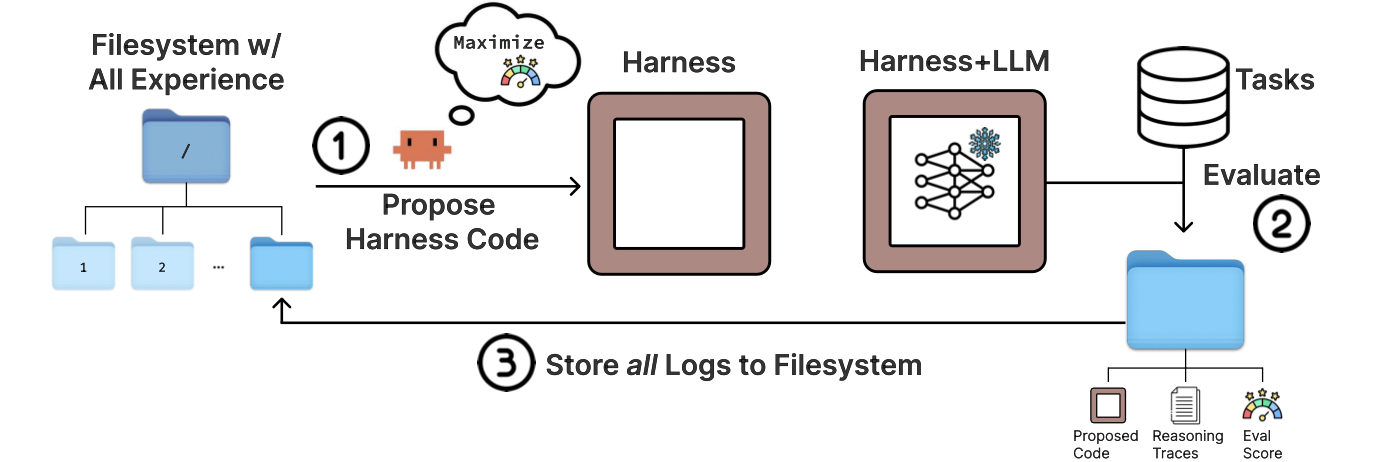
\includegraphics[width=\linewidth]{figures/metaharness.png}
    \caption{元框架方法示意 \citep{lee2026meta}}
    \label{fig:metaharness}
\end{figure}

元框架 \citep{lee2026meta} 同样取得了良好结果，它使用外部记忆与文本优化。图~\ref{fig:metaharness} 展示了元框架如何工作。（1）一个文件系统存放了此前所有候选的源代码、执行轨迹与分数；智能体读取这些内容，并为新框架生成代码。（2）所提出的框架在评估任务上被评估。（3）所有提出的代码、推理轨迹与评估分数都被存入文件系统中的一个新目录，循环随之重复。

自我框架 \citep{zhang2026self} 与智能体框架工程 \citep{lin2026agentic} 进一步探索了框架设计，在软件工程任务上取得了显著改进。递归自我演化智能体 \citep{nguyen2026recursive} 则聚焦于自我改进型智能体的选择方面。

\citet{luo2026autodesign} 描述了另一个用例。他们用元框架设计了一个把科学论文转成会议海报的框架。因此这项工作在两个层面都有贡献：一套制作元框架的方法，以及一个用于设计海报的具体框架——作者显然把它用在了自己的论文上。

\begin{figure}
    \centering
    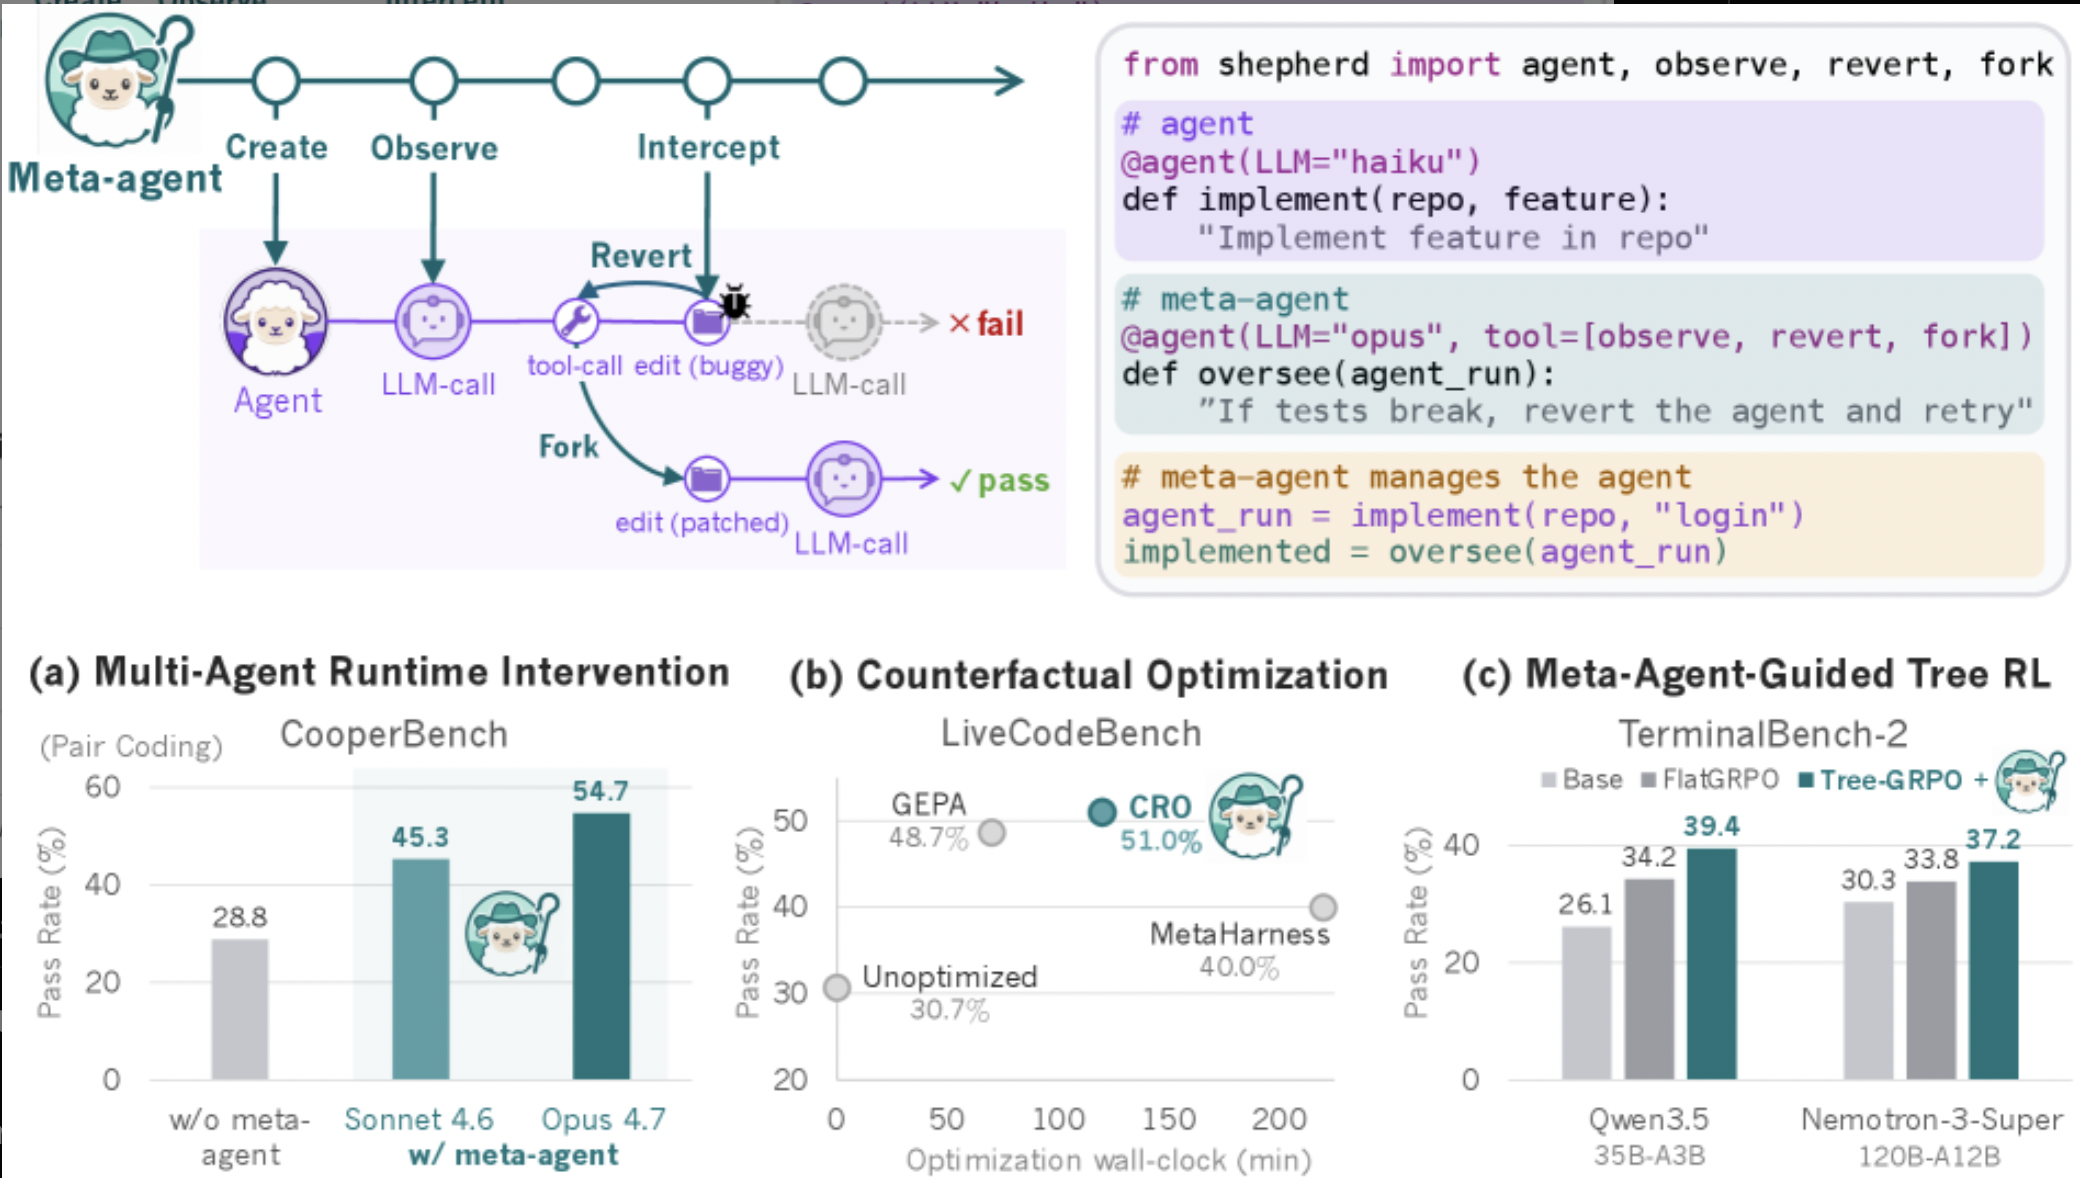
\includegraphics[width=\linewidth]{figures/shepherd.png}
    \caption{Shepherd 元智能体环境示意 \citep{yu2026shepherd}}
    \label{fig:shepherd}
\end{figure}

Shepherd 系统 \citep{yu2026shepherd} 提供了一个可用的元智能体编程环境。\footnote{\url{https://shepherd-agents.ai}} Shepherd 把大语言模型智能体定义为 Python 函数，从而可以监控智能体的执行轨迹，并进行回滚、分叉、修改与恢复。早期实验显示，它在三个不同基准上都带来了显著的性能提升，如图~\ref{fig:shepherd} 所示。

\citet{ren2026self} 是一篇综述，涵盖自我改进型智能体设计的更多方法。其分类法明确识别出了双层架构。
\section{结语}
本章我们讨论了一些高级架构，既有 Transformer 层面的，也有智能体层面的。两者都是极为活跃的研究领域。

\bibliographystyle{plainnat}
\bibliography{agenticbook,refs,case,synthetic}
